%%%%%%%%%%%%%%%%%%%%%%%%%%%%%%%%%%%%%%%%%%%%%%%%%%%%%%%%%%%%%%%%%%%%%%%%
%%% Double-blind submission (authors hidden). For the camera-ready
%%% version, switch to the second line.
\documentclass[sigconf,anonymous]{aamas}
%\documentclass[sigconf]{aamas}

%%%%%%%%%%%%%%%%%%%%%%%%%%%%%%%%%%%%%%%%%%%%%%%%%%%%%%%%%%%%%%%%%%%%%%%%
%%% Packages (acmart already loads amsmath, graphicx, booktabs, hyperref,
%%% xcolor and natbib)
%%%%%%%%%%%%%%%%%%%%%%%%%%%%%%%%%%%%%%%%%%%%%%%%%%%%%%%%%%%%%%%%%%%%%%%%

\usepackage{balance}        % balance the columns of the last page
\usepackage{xspace}
\usepackage{multirow}
\usepackage{subcaption}
\usepackage{enumitem}
\usepackage[capitalise,noabbrev]{cleveref}
\usepackage{tikz}
\usetikzlibrary{arrows.meta,positioning,fit,calc}
\usepackage[printonlyused,withpage]{acronym}
\usetikzlibrary{backgrounds}   % o template já carrega arrows.meta, positioning, fit, calc
\usepackage{algorithm}
\usepackage{algpseudocode}
% Permit modest extra interword flexibility before accepting an overfull line.
\setlength{\emergencystretch}{1em}
%%%%%%%%%%%%%%%%%%%%%%%%%%%%%%%%%%%%%%%%%%%%%%%%%%%%%%%%%%%%%%%%%%%%%%%%
%%% AAMAS-2027 copyright block (do not change)
%%%%%%%%%%%%%%%%%%%%%%%%%%%%%%%%%%%%%%%%%%%%%%%%%%%%%%%%%%%%%%%%%%%%%%%%

\makeatletter
\gdef\@copyrightpermission{
  \begin{minipage}{0.2\columnwidth}
   \href{https://creativecommons.org/licenses/by/4.0/}{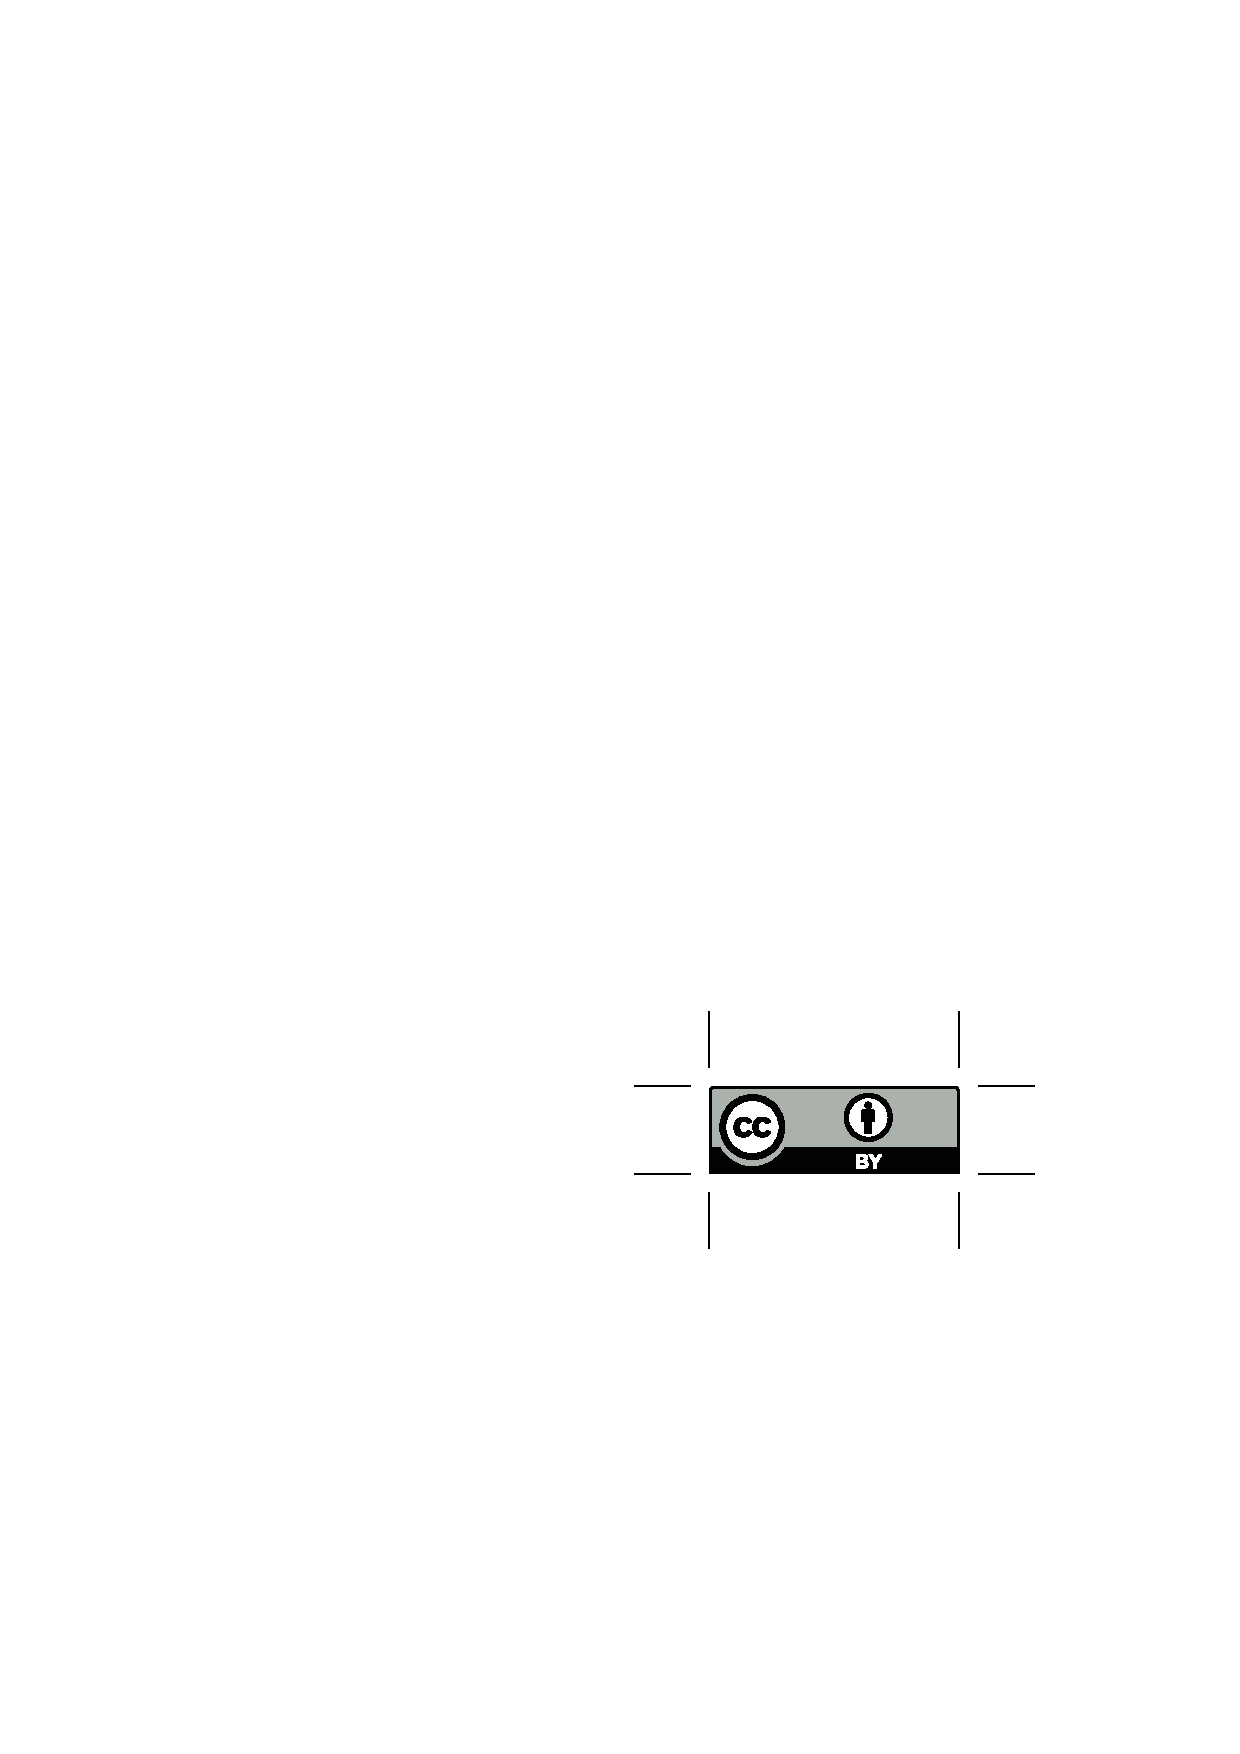
\includegraphics[width=0.90\textwidth]{by}}
  \end{minipage}\hfill
  \begin{minipage}{0.8\columnwidth}
   \href{https://creativecommons.org/licenses/by/4.0/}{This work is licensed under a Creative Commons Attribution International 4.0 License.}
  \end{minipage}
  \vspace{5pt}
}
\makeatother

\setcopyright{ifaamas}
\acmConference[AAMAS 2027]{Proc.\@ of the 26th International Conference
on Autonomous Agents and Multiagent Systems (AAMAS 2027)}{3--7 May 2027}{Hanoi, Vietnam}{M.~Baldoni, F.~Fang, W.~Yeoh, N.~Yorke-Smith (eds.)}
\copyrightyear{2027}
\acmYear{2027}
\acmDOI{}
\acmISBN{}

\acmSubmissionID{<<OpenReview submission id>>}
\submissionType{Research Paper Track}

%%%%%%%%%%%%%%%%%%%%%%%%%%%%%%%%%%%%%%%%%%%%%%%%%%%%%%%%%%%%%%%%%%%%%%%%
%%% Macros
%%%%%%%%%%%%%%%%%%%%%%%%%%%%%%%%%%%%%%%%%%%%%%%%%%%%%%%%%%%%%%%%%%%%%%%%

%% Method name in one place, so a rename is a one-line change.
\newcommand{\sys}{WitnessRAG\xspace}

%% Pipeline operations (small caps in the text).
\newcommand{\op}[1]{\textsc{#1}\xspace}
\newcommand{\register}{\op{Register}}
\newcommand{\search}{\op{Search}}
\newcommand{\plan}{\op{Plan}}
\newcommand{\prove}{\op{Prove}}
\newcommand{\verify}{\op{Verify}}
\newcommand{\respond}{\op{Respond}}

%% Relations and variables in examples: \rel{camped\_at}(Melanie, \var{where}).
\newcommand{\rel}[1]{\textsf{#1}}
\newcommand{\var}[1]{\textsf{?#1}}

%% Notation shared by the method and the problem formulation.
\newcommand{\mem}{\mathcal{M}}          % memory
\newcommand{\facts}{\mathcal{F}}        % fact base
\newcommand{\passages}{\mathcal{D}}     % passages (chunks)
\newcommand{\witness}{W}                % a witness
\newcommand{\ctx}{C}                    % reader context
\newcommand{\kread}{k}                  % reader budget (passages)
\newcommand{\kwit}{k_W}                 % passages a witness may replace
\DeclareMathOperator{\score}{score}
\DeclareMathOperator{\simil}{sim}
\DeclareMathOperator{\imp}{imp}
\DeclareMathOperator{\prox}{prox}

%% Writing aids. Remove every \todo before submission:
%% grep -n "\\todo" sections/*.tex
\newcommand{\todo}[1]{\textcolor{red}{[TODO: #1]}}
\newcommand{\BibTeX}{\rm B\kern-.05em{\sc i\kern-.025em b}\kern-.08em\TeX}

%%%%%%%%%%%%%%%%%%%%%%%%%%%%%%%%%%%%%%%%%%%%%%%%%%%%%%%%%%%%%%%%%%%%%%%%
%%% Acronyms: \ac{LLM} expands on first use, \acp{LLM} is the plural.
%%%%%%%%%%%%%%%%%%%%%%%%%%%%%%%%%%%%%%%%%%%%%%%%%%%%%%%%%%%%%%%%%%%%%%%%

\acrodef{LLM}{large language model}
\acrodef{RAG}{retrieval-augmented generation}
\acrodef{KG}{knowledge graph}
\acrodef{QA}{question answering}
\acrodef{PPR}{Personalized PageRank}
\acrodef{RRF}{reciprocal rank fusion}
\acrodef{AOT}{ahead-of-time}
\acrodef{JIT}{just-in-time}
\acrodef{NER}{named entity recognition}
\acrodef{OpenIE}{open information extraction}

%%%%%%%%%%%%%%%%%%%%%%%%%%%%%%%%%%%%%%%%%%%%%%%%%%%%%%%%%%%%%%%%%%%%%%%%
%%% Title and authors
%%%%%%%%%%%%%%%%%%%%%%%%%%%%%%%%%%%%%%%%%%%%%%%%%%%%%%%%%%%%%%%%%%%%%%%%

% \title[Show Me the Witness: Proof-Grounded Retrieval for Long-Term Memory in LLM Agents]{Show Me the Witness: Proof-Grounded Retrieval for Long-Term Memory in LLM Agents}

\title[WitnessRAG: Long-Term Memory Retrieval for LLM Agents through Witness Search]{WitnessRAG: Long-Term Memory Retrieval for LLM Agents through Witness Search}



\author{Rodrigo Gonçalves Flexa}
\orcid{0009-0006-7591-7560}
\affiliation{
  \department{Institute of Computing}
  \institution{University of Campinas (UNICAMP)}
  \city{Campinas}
  \state{São Paulo}
  \country{Brazil}}
\email{ra299214@dac.unicamp.br}

\author{Luiz Eduardo Assunção de Albuquerque}
\affiliation{
  \department{Department of Mathematical Sciences, Faculty of Sciences}
  \institution{University of Lisbon}
  \city{Lisbon}
  \country{Portugal}}
\email{fc62505@alunos.ciencias.ulisboa.pt}

\author{Leandro A. Villas}
\orcid{0000-0002-3372-3366}
\affiliation{
  \department{Institute of Computing}
  \institution{University of Campinas (UNICAMP)}
  \city{Campinas}
  \state{São Paulo}
  \country{Brazil}}
\email{villas@ic.unicamp.br}

\author{Julio Cesar dos Reis}
\orcid{0000-0002-9545-2098}
\affiliation{
  \department{Institute of Computing}
  \institution{University of Campinas (UNICAMP)}
  \city{Campinas}
  \state{São Paulo}
  \country{Brazil}}
\email{jreis@ic.unicamp.br}

\renewcommand{\shortauthors}{Flexa et al.}

\begin{abstract}
Long-term conversational memory requires agents to answer questions
whose support is scattered across sessions and anchored in time.
Retrieval methods that rank memories individually can return records
that are each relevant to the question yet fail to connect into an
answer. We present \sys, a retrieval framework that casts memory access
as \emph{witness search}: finding a set of stored facts that jointly
satisfies the relational requirements of a question. \sys organizes the
interaction history into a graph of dated propositions linked to the
dialogue from which they were extracted. At query time, a language
model grounds a conjunctive plan in retrieved evidence, and an executor
searches the graph, without model calls, for facts that satisfy
the plan under consistent variable bindings. Unsatisfied requirements
and rejected candidates are returned to the planner, while a
question-dependent temporal reference adapts ranking to the period the
question concerns. Accepted witnesses then guide the construction of a
compact context for the reader. By separating the specification of what
must be found from the computation of how stored facts connect, \sys
grounds each answer in evidence that can be traced back to the original
conversation.

% Add empirical findings once the evaluation is complete and validated.

\end{abstract}

\ccsdesc[500]{Computing methodologies~Intelligent agents}
\ccsdesc[300]{Computing methodologies~Natural language processing}
\ccsdesc[300]{Information systems~Retrieval models and ranking}

\keywords{LLM Agents, Agent Memory, Retrieval-Augmented Generation,
Data Provenance, Knowledge Graphs, Long-Term Conversational Memory}

%%%%%%%%%%%%%%%%%%%%%%%%%%%%%%%%%%%%%%%%%%%%%%%%%%%%%%%%%%%%%%%%%%%%%%%%

\begin{document}

\maketitle

\section{Introduction}
\label{sec:intro}

Agents built on \acp{LLM} rely on long-term memory to retain information
across interactions, in settings ranging from personal assistance to
simulated societies and multi-episode
tasks~\cite{park2023generative,packer2023memgpt,sumers2024coala,zhang2025survey}.
Interaction histories quickly exceed the context window, and even within
it, a model's use of information degrades with context length and
position~\cite{liu2024lost,hsieh2024ruler}. External memory removes the
capacity constraint but introduces a retrieval problem: given a question,
which stored evidence should the agent read?

The problem is hardest when the answer depends on facts recorded in
different sessions, connected through intermediate entities, or tied to
a particular period. Long-term conversational benchmarks are built
around precisely these forms of cross-session and temporal
reasoning~\cite{maharana2024locomo,wu2025longmemeval}. Consider a question
such as \emph{``Where did Melanie go camping after she adopted her dog?''}
Answering it requires two facts, possibly mentioned weeks apart, and the
temporal relation between them. The fact about the adoption may bear
little lexical resemblance to the question, whereas many camping-related
memories may resemble it closely without being the right ones. Relevance,
in this setting, is a property of \emph{sets} of memories rather than of
individual records.

Existing approaches address this challenge in two ways. Ranking methods
score memory records, or propagate relevance through a structured store,
before selecting a bounded
context~\cite{park2023generative,zhong2024memorybank,chhikara2025mem0,gutierrez2024hipporag}.
Their selection criteria, however, do not test whether the retrieved
records jointly satisfy the relations the answer requires. Iterative
methods let intermediate reasoning guide further
retrieval~\cite{trivedi2023ircot,asai2024selfrag,jeong2024adaptiverag,yan2025gam}.
They can revise the search as evidence accumulates, but a model's judgment
that the evidence is sufficient does not identify which facts support
the answer or how they connect.

We argue that these relational requirements should be stated and executed
explicitly. Conjunctive queries offer a natural formalism: a query
specifies relations whose arguments must admit a consistent
assignment~\cite{chandra1977conjunctive}, and a \emph{witness} is a set of
facts that realizes one such assignment, thereby explaining the answer
through its provenance~\cite{buneman2001why,green2007provenance}. Applied
to memory, this perspective separates two tasks of different nature. The
linguistic task of deciding \emph{what} to find is left to a language
model; the combinatorial task of finding facts that jointly meet that
specification is delegated to an executor.

Building on this idea, we introduce \sys, a retrieval framework for
long-term agent memory. \sys organizes the interaction history into a
graph of dated propositions that remain linked to their source dialogue.
Given a question, a language model writes a conjunctive plan grounded in
retrieved evidence, and an executor searches the graph for witnesses of
that plan. When search fails or a candidate is rejected, the unsatisfied
requirement tells the planner what to revise. Accepted witnesses finally
guide the selection of the evidence passed to the reader. Because each
answer is tied to an explicit derivation over stored facts, retrieval
becomes inspectable: one can see not only what was retrieved, but why it
supports the answer.

This paper makes the following contributions:
\begin{itemize}
  \item We formulate long-term memory retrieval as \emph{witness search}
    over conjunctive plans, separating the interpretation of a question
    from the execution of its relational requirements.
  \item We present \sys, a retrieval controller that combines
    evidence-grounded planning, reference-relative temporal ranking,
    consistent-binding search, and verification with gap-driven
    replanning.
  \item We show how witnesses can guide the construction of a compact,
    source-linked reader context composed of dated propositions and
    passage summaries.
\end{itemize}
% Add empirical contributions only after validating the completed runs,
% comparison protocol, uncertainty estimates, and reported configuration.

The remainder of the paper is organized as follows.
\Cref{sec:background} reviews the formal background and related work.
\Cref{sec:problem} formulates the task and \cref{sec:method} presents
\sys. \Cref{sec:setup,sec:results} describe the evaluation, and
\cref{sec:discussion,sec:conclusion} discuss limitations and conclude
the paper.

\section{Background}
\label{sec:background}

\subsection{Preliminaries}
\label{sec:preliminaries}

Conjunctive queries express information needs as relations that must
hold jointly. Over binary relations, a query takes the form
\begin{equation}
 Q(x)=\exists\bar y\;\bigwedge_{j=1}^{m}r_j(t_j,t'_j),
 \label{eq:cq}
\end{equation}
where each term is a constant or a variable, $x$ is the answer variable,
and $\bar y$ collects the remaining
variables~\cite{chandra1977conjunctive}. An answer is obtained by an
assignment of values to variables under which every atom matches a
stored fact, with all occurrences of a variable receiving the same value.

A \emph{witness} for an answer is a set of facts that suffices to derive
it: evaluating the query over those facts alone yields the
answer~\cite{buneman2001why}. A witness contains at most $m$ facts, and
an answer may admit several witnesses; provenance semirings capture these
alternative derivations~\cite{green2007provenance}. For retrieval, this
notion provides a structural target: a set of facts that jointly
satisfies the query, rather than a list of facts that are individually
relevant to it.

\subsection{Related Work}
\label{sec:related}

\paragraph{Memory architectures for LLM agents.}
Agent memory systems manage long interaction histories through virtual
context management~\cite{packer2023memgpt,lee2024readagent}, memory
streams with reflection or forgetting~\cite{park2023generative,zhong2024memorybank},
and feedback accumulated across
episodes~\cite{shinn2023reflexion,flexa2026bridging}. Other architectures
maintain extracted facts~\cite{chhikara2025mem0}, linked
notes~\cite{xu2025amem}, temporal
graphs~\cite{rasmussen2025zep,anokhin2025arigraph}, hierarchical
stores~\cite{kang2025memoryos,zhang2025gmemory}, or compressed and
enriched records~\cite{fang2026lightmem,liu2026simplemem,salama2025meminsight}.
These works primarily concern how memory is \emph{represented}. \sys is
complementary: it addresses how the relational requirements of a question
should drive retrieval from such a representation.

\paragraph{Graph-based and iterative retrieval.}
Structured retrieval exploits relations to reach information beyond
direct similarity to the question, through community
summaries~\cite{edge2024graphrag}, recursive summary
trees~\cite{sarthi2024raptor}, or relevance propagation over open
knowledge graphs~\cite{gutierrez2024hipporag,gutierrez2025hipporag2}.
Iterative approaches interleave retrieval with
reasoning~\cite{trivedi2023ircot}, let a language model explore a
graph~\cite{sun2024tog}, or adapt retrieval to the
input~\cite{asai2024selfrag,jeong2024adaptiverag}. In agent memory,
MemAgent learns memory operations through reinforcement
learning~\cite{yu2026memagent}, and GAM employs a researcher agent that
searches stored pages and reflects on whether further search is
needed~\cite{yan2025gam}. \sys shares the iterative character of these
methods but differs in where composition happens: the language model
states the query, and the bindings and supporting facts are computed by
an executor whose failures are returned to the planner as explicit
feedback.

\paragraph{Temporal memory.}
Time enters memory systems either as a retrieval preference or as an
attribute of stored information. Generative Agents score memories by
recency~\cite{park2023generative}, MemoryBank models forgetting over
elapsed time~\cite{zhong2024memorybank}, Zep attaches temporal validity
to graph relations~\cite{rasmussen2025zep}, and Zero-Mem organizes
evidence along temporal structure~\cite{xiao2026zeromem}. Recency,
however, captures only one kind of temporal need: a question may concern
a first occurrence or a specific past period. \sys lets each question
define its own temporal reference and treats proximity to it as a soft
preference rather than a hard constraint.

\paragraph{Provenance, attribution, and verification.}
Database provenance characterizes the facts that contribute to a query
answer~\cite{buneman2001why,green2007provenance}. For language models,
attribution links generated claims to source passages~\cite{gao2023alce},
and verification uses targeted questions to detect and revise unsupported
claims~\cite{dhuliawala2024cove}. \sys brings provenance into retrieval
itself: a witness identifies the source utterances against which a
candidate answer is verified and from which the reader's context is
built, making the supporting derivation available for inspection.

\section{Task Formulation}
\label{sec:problem}

An agent accumulates an interaction history $H=(s_1,\ldots,s_T)$ of dated
dialogue sessions. A memory construction process maps this history to a
memory $\mem$ comprising the source passages and representations derived
from them. Given a question $q$, retrieval constructs a context $\ctx$
under a budget $b$, from which a reader produces an answer:
\begin{equation}
 \ctx=\mathrm{Retrieve}(q,\mem;b),\qquad
 \hat a=\mathrm{Read}(q,\ctx).
 \label{eq:task}
\end{equation}
The budget bounds the evidence delivered to the reader, so the goal of
retrieval is to select evidence that \emph{supports} a correct answer,
rather than records that merely resemble the question.

We consider questions whose relational requirements can be expressed as
a conjunctive query (\cref{sec:preliminaries}). Under this view,
retrieval amounts to finding witnesses of the query in memory, with the
temporal scope and expected form of the answer shaping which witnesses
are preferred. The formulation thus distinguishes two responsibilities:
\emph{interpreting} the question as a query, and \emph{satisfying} that
query over stored facts. Witnesses make the second responsibility
explicit and checkable; their adequacy for the original question still
depends on the interpretation and on the stored facts, a point we return
to in \cref{sec:discussion}.

\section{\texorpdfstring{\sys}{WitnessRAG}}
\label{sec:method}

\sys treats memory retrieval as the search for facts that jointly satisfy
the information requirements of a question. It operates in two stages
(\cref{fig:overview}). \emph{Memory construction} organizes the
interaction history into a graph of dated propositions linked to their
source passages. \emph{Memory retrieval} grounds a plan in retrieved
evidence, searches the graph for witnesses of that plan, verifies them,
and assembles a compact context for the reader. Throughout, the planner
specifies \emph{what} must be found, and the executor determines
\emph{how} stored facts connect to satisfy it.

\begin{figure*}[t]
  \centering
  \includegraphics[width=\textwidth]{figures/overview-standalone.pdf}
  \caption{\textbf{Overview of \sys.}
  (1) \emph{Memory construction}: dialogue histories are turned into
  dated propositions, stored both as statements and as graph triples
  linked to their source utterances. (2) \emph{Memory retrieval}: a
  planner grounded in retrieved evidence specifies the relational
  requirements of the question, its answer type, and a temporal reference.
  An executor searches the graph for witnesses under consistent bindings;
  a verifier checks candidates against their sources, and gaps or
  rejections are fed back to the planner. Accepted witnesses guide the
  selection of propositions and passage summaries passed to the reader.
  Blue outlines denote LLM operations, green outlines denote retrieval or
  deterministic processing, dotted links denote provenance, and dashed
  arrows denote feedback.}
  \Description{The architecture has two stages: memory construction and memory retrieval. Memory construction
  extracts propositions and indexes their time and importance metadata.
  Source passages and the dated proposition graph are connected by
  provenance. A question triggers evidence retrieval and an LLM planner.
  The planner specifies conjunctive requirements, answer type, temporal
  reference and weights. A graph executor finds consistent bindings without
  LLM calls. A conditional verifier checks source utterances, returning
  gaps or rejections to the planner. Accepted support and relevance-ranked
  candidates guide context selection. The reader receives dated statements
  and passage summaries and generates an answer.}
  \label{fig:overview}
\end{figure*}


\subsection{Memory Construction}
\label{sec:method-register}

The memory pairs a passage store $\passages$ with a fact graph
$\mathcal G=(\mathcal N,\facts)$. Passages preserve the original dialogue
and its session structure. From them, an \ac{LLM} extracts
self-contained propositions, each represented both as a natural-language
statement and as a subject--relation--object triple: the statement is
what the reader consumes, and the triple is what the executor searches.
Entity normalization merges recurring mentions, so that facts recorded
in different sessions can take part in the same derivation.

Each fact is annotated with an event interval, an importance score, and a
link to its source utterance. Temporal expressions are resolved relative
to the session in which they occur, which distinguishes when an event
happened from when it was mentioned. Importance is a
question-independent estimate of the salience expressed in the source
utterance. We write $\mem=(\passages,\facts)$ for the resulting memory
and $\mathrm{src}(W)$ for the source passages of a set of facts $W$.
These provenance links allow any witness to be traced back to the
utterances from which its facts were extracted. Construction is performed
once per history and shared across all questions about it.

\subsection{Evidence-Grounded Planning}
\label{sec:method-plan}

Retrieval starts with a hybrid dense--lexical search, fused by
\ac{RRF}, that yields an initial pool of evidence. The planner, an
\ac{LLM}, receives the question together with dated facts from this pool
and the relations and entities available in memory. Planning
\emph{after} an initial retrieval lets the model phrase its query in the
vocabulary of the stored history rather than that of the question.

A plan $\pi$ consists of a conjunctive query in the form of \cref{eq:cq},
the expected answer type (e.g., an entity, a date, or a set of values),
a temporal reference, and ranking weights. Shared variables encode
dependencies between facts: the value that satisfies one atom constrains
the facts that can satisfy another. Operations such as comparison or
date arithmetic are not executed over the graph; the plan retrieves
their premises, and the reader performs them.

The temporal reference designates the period against which memories are
ranked: the present, the beginning of the history, or an interval named
in the question. Together with the weights, it allows the same memory to
be searched differently for questions about recent events, first
occurrences, or specific periods. Once a plan is available, the evidence
pool is expanded under the corresponding ranking.

\subsection{Reference-Relative Ranking}
\label{sec:method-score}

Passage retrieval and witness search share a scoring function that
combines relevance, importance, and temporal proximity:
\begin{equation}
 s(x\mid q,\pi)=
 \lambda_s\,\mathrm{sim}(x)
 +\lambda_i\,\kappa_x
 +\lambda_t\,g(x;\rho),
 \label{eq:score}
\end{equation}
where $\kappa_x$ is the importance of item $x$, $\rho$ is the temporal
reference of $\pi$, and the nonnegative weights, chosen by the planner,
sum to one. For a passage, $\mathrm{sim}(x)$ is its normalized retrieval
score; for a fact, it measures how well the fact matches the
corresponding query atom.

Temporal proximity decays with the distance between the event interval
$I_x$ and the reference:
\begin{equation}
 g(x;\rho)=\exp\!\left(-\frac{\delta(I_x,\rho)}{h_\rho}\right),
 \label{eq:proximity}
\end{equation}
where $\delta$ vanishes for overlapping intervals and otherwise measures
their separation, and $h_\rho$ sets the decay scale. With the present as
reference, \cref{eq:proximity} reduces to recency; with an earlier
reference, it favors events near that period. Time thus acts as a
question-dependent preference rather than a universal bias toward recent
memories.

\subsection{Witness Search}
\label{sec:method-prove}

The executor searches for witnesses of the planned query without invoking
a language model. As defined in \cref{sec:preliminaries}, a witness is a
set of facts that instantiates every atom under a single consistent
assignment. Matching is semantic rather than exact, which absorbs
differences between the planner's phrasing and the stored propositions;
consistency is strict, so that once a variable is bound, all subsequent
atoms must agree with it. This prevents facts that are individually
plausible from being combined into an incoherent answer.

Search explores partial assignments with a bounded beam, starting from
the most constrained atoms. For a witness $W=\{f_1,\ldots,f_m\}$, where
$f_j$ matches the $j$-th atom, the search minimizes
\begin{equation}
 J(W)=-\sum_{j=1}^{m}\log s(f_j\mid q,\pi)
       +\gamma\,|\mathrm{src}(W)|.
 \label{eq:witness-search}
\end{equation}
The first term favors derivations whose atoms are all well matched, since
a single weak link dominates the sum; the second discourages support
that is dispersed across unnecessarily many passages. A candidate is
accepted only when its matching strength is sufficient on its own, so
that temporal or importance preferences can reorder plausible witnesses
but cannot rescue a poor match. For set-valued answers, support is
assessed separately for each member.

When no consistent extension exists, search reports the unsatisfied atom
together with the bindings established so far. This \emph{gap} states
precisely which requirement remains unresolved and gives the planner a
concrete target for revision.

\subsection{Verification and Replanning}
\label{sec:method-verify}

Witness search establishes that stored facts satisfy the plan, but not
that the plan and the extracted facts faithfully reflect the dialogue.
A verifier therefore checks candidate answers against the source
utterances of their witnesses, assessing whether the evidence concerns
the intended entity, period, and answer type. Members of a set-valued
answer are verified individually, so that a subset can be retained.
Verification is applied selectively, when the support is not already
evident in the retrieved evidence.

If no candidate is accepted, the gaps and the verifier's feedback are
returned to the planner, which may revise a relation, an entity, or the
temporal interpretation before the executor searches again
(\cref{alg:search}). The cycle ends when a witness is accepted or the
cycle budget is exhausted, in which case retrieval falls back to
relevance ranking alone.

\begin{algorithm}[t]
\caption{Witness-guided memory retrieval}
\label{alg:search}
\small
\begin{algorithmic}[1]
\Require Question $q$, memory $\mem$, cycle limit $R$, context budget $b$
\State $E\gets\search(q,\mem)$; $\Delta\gets\emptyset$; $W^+\gets\emptyset$
\For{$c=1,\ldots,R$}
  \State $\pi\gets\plan(q,E,\Delta)$
  \State $E\gets E\cup\search(q,\mem;\pi)$
  \State $(W,\Delta)\gets\prove(\pi,\mem,E)$
  \State $(W^+,\Delta)\gets\verify(q,\pi,W,\Delta)$
  \If{$W^+\neq\emptyset$} \State \textbf{break} \EndIf
\EndFor
\State $\ctx\gets\op{Assemble}(q,\mem,\pi,W^+,b)$
\State \Return $\mathrm{Read}(q,\ctx)$
\end{algorithmic}
\end{algorithm}

\subsection{Context Assembly and Cost}
\label{sec:method-respond}
\label{sec:method-guarantees}

The reader's context combines dated propositions with summaries of their
source passages. Propositions are selected by their membership in
accepted witnesses and by their relevance to the question and the plan,
favoring coverage over redundancy within the budget $b$. They are grouped
by session and annotated with their event dates, while passage summaries,
computed independently of the question and reused across queries,
restore surrounding context that individual propositions omit. Witnesses
thus prioritize evidence without excluding other relevant material. The
reader formulates the answer and carries out any comparison or date
arithmetic the plan has deferred to it.

With at most $R$ cycles, retrieval issues at most $R$ planning and $R$
verification calls, followed by a single reader call; graph execution
requires none. Extraction and summarization are one-time costs amortized
over all questions on the same history. Language models are thus used
where interpretation is required, namely in planning, verification, and
answer generation, while relational composition is carried out by the
executor.

%%% ====================================================================
%%% 5. Experimental Setup
%%% --------------------------------------------------------------------
%%% Protocol of GAM (Yan et al., 2025): LoCoMo (F1, BLEU-1; 1,540
%%% questions, adversarial excluded); HotpotQA 56K/224K/448K (F1); RULER
%%% 128K (Retri., MT, AGG., QA accuracy); NarrativeQA (F1, 300 questions).
%%% Same reader, BGE-M3, 2,048-token passages and top-5 for every method.
%%% Backbones: GPT-4.1-mini and Qwen2.5-14B-Instruct.
%%% ====================================================================
\section{Experimental Setup}
\label{sec:setup}

\subsection{Benchmarks and Metrics}
\label{sec:setup-benchmarks}

\subsection{Baselines}
\label{sec:setup-baselines}

\subsection{Implementation Details}
\label{sec:setup-implementation}


%%% ====================================================================
%%% 6. Results and Analysis
%%% --------------------------------------------------------------------
%%% Main table on LoCoMo (per category, F1 / BLEU-1, two backbones);
%%% long-context table in the layout of GAM's Table 1(b); ablations (one
%%% design decision per row); reader-budget sweep (k = 1..5) and cost
%%% (LLM calls and tokens per question); a worked example.
%%% ====================================================================
\section{Results and Analysis}
\label{sec:results}

\subsection{Main Results on LoCoMo}
\label{sec:results-locomo}

\subsection{Long-Context Benchmarks}
\label{sec:results-longctx}

\subsection{Ablation Study}
\label{sec:results-ablation}

% \subsection{Reader Budget and Cost}
% \label{sec:results-budget}

% \subsection{Case Study}
% \label{sec:results-case}


\section{Discussion and Limitations}
\label{sec:discussion}

\paragraph{Relational support.}
Witnesses make explicit the connections that support an answer, but
their adequacy for the original question depends on the extracted facts
and on the planner's interpretation. Semantic matching and source
verification accommodate linguistic variation, yet both remain
approximate. Moreover, support for each member of an answer set does not
establish that the set is complete. These observations motivate
evaluating not only answer quality but also the evidence offered for
each answer.

\paragraph{Temporal interpretation.}
Reference-relative ranking adapts retrieval to the period a question
concerns, but its effectiveness is bounded by the quality of the dates
inferred from dialogue, especially when event times are implicit.
Temporal proximity is a ranking preference rather than a temporal
reasoning formalism: ordering and comparison are still left to the
reader.

\paragraph{Compression and cost.}
Propositions provide a compact view of the history, and passage summaries
restore part of the surrounding context. This compression trades
coverage for detail: under a tight budget, part of an accepted witness
may not reach the reader, so finding support does not guarantee
delivering it in full. A fair comparison should therefore account for
the context actually read and its token cost, including the one-time
cost of extraction and summarization amortized across questions.

\section{Conclusion}
\label{sec:conclusion}

We presented \sys, a retrieval framework that makes the relational
requirements of a question explicit in long-term agent memory. By
separating the interpretation of a question, performed by a language
model, from the search for facts that jointly satisfy it, performed by
an executor over dated and source-linked propositions, \sys ties each
answer to a derivation that can be inspected and verified. Execution
gaps and verification feedback turn failures into concrete guidance for
replanning, and witnesses shape the context delivered to the reader.
Future work includes richer temporal constraints within the query
language and tighter coupling between witness support and the reader's
context budget.


%%% Omitted automatically in anonymous mode.
\begin{acks}
%%% Printed only in the camera-ready version (hidden in anonymous mode).
\todo{Funding agencies and grant numbers.}

\end{acks}

%%% Issue \balance in the first column of the last page (camera-ready).
%\balance

\bibliographystyle{ACM-Reference-Format}
\bibliography{references}

%%% Supplementary material (separate PDF, not counted in the 8 pages):
%%% compile sections/appendix.tex in its own file if needed.

\end{document}
